{\textbf{1.立即寻址}}

这个寻址方式直接给出操作数,不需要给出地址去其他地方找操作数。也就是说,下图中的A不是操作数的地址,而\textbf{就是操作数本身}。通常把``\#''符号放在立即数前面,以表示该寻址方式为立即寻址,如\textbf{\#20H}。其他寻址方式则不用特殊符号来表示。

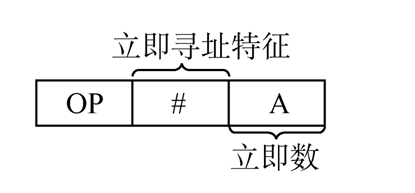
\includegraphics[width=2.08333in,height=0.96875in]{png-jpeg-pics/1217CD46D18068794B47170C8560B3F8.png}

{\textbf{2.直接寻址}}

首先将一个生活实例作为铺垫。就好像从淘宝购物,有些快递是直接送上门的,就类似于立即寻址,而有些快递是送到一个固定地点,然后发短信告诉客户,客户再去取。\textbf{短信上的地址就是直接寻址中给出的地址,通过这个地址客户就可以拿到他们的物品(操作数)。}也就是说,取到操作数之后再将操作数送往运算器或其他地方。可见,直接寻址在执行阶段需要访问一次存储器去取操作数,如下图所示。

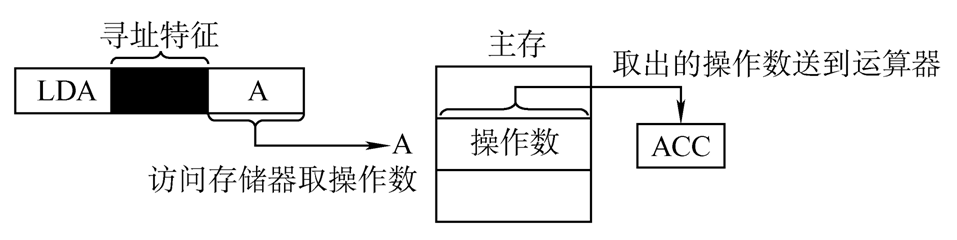
\includegraphics[width=6in]{png-jpeg-pics/316231AD55846BF7C576AA754E41385C.png}

{\textbf{3.隐含寻址(了解即可)}}

隐含寻址指指令字中不明显地给出操作数地址,其操作数地址隐含在操作码或者某个寄存器中。其中最典型的例子就是一地址格式的加法指令,如下图所示。操作码显示的是ADD,说明肯定至少需要两个操作数才能做加法运算,而地址码仅仅给出了一个操作数的地址,那另外一个操作数呢?没错,就在ACC(累加器)中(这个没有为什么,就是规定)。换句话说,\textbf{一地址格式的算术运算指令的另外一个操作数隐含在ACC中。}

\textbf{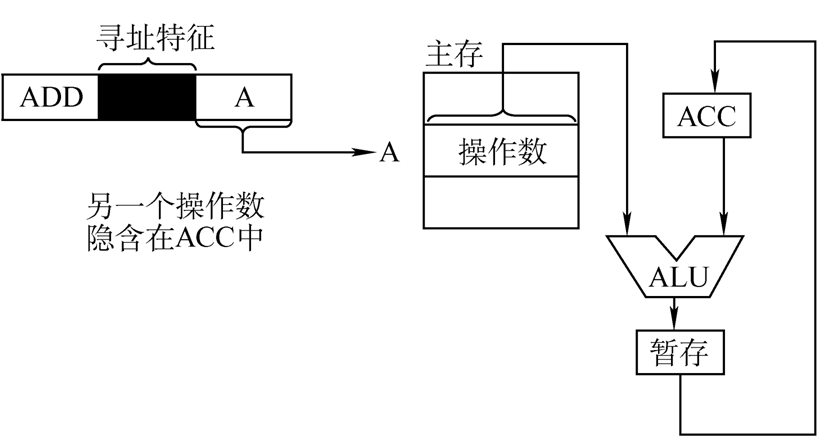
\includegraphics[width=6in]{png-jpeg-pics/3930ABDAB3E51036A984314FE155DF51.png}\\
}

{\textbf{4.间接寻址(非常重要)}}

直接寻址是直接给出了操作数的有效地址,即直接可以通过该地址找到操作数,但间接寻址指令给出的地址是操作数有效地址的地址。{间接寻址又分为}\textbf{一次间接寻址和多次间接寻址。}

{\textbf{5.寄存器寻址}}

寄存器寻址比较简单,基本和直接寻址类似。在直接寻址的指令字中,地址码字段给出的是主存的地址,而在寄存器寻址的指令字中,地址码字段直接给出了寄存器编号Ri,则\textbf{操作数的有效地址EA=Ri。}

{\textbf{6.寄存器间接寻址}}

和寄存器寻址的不同之处在于,Ri的内容不是操作数,而是操作数所在主存单元的地址号(很容易出选择题),即\textbf{有效地址EA=(Ri)。}

{\textbf{7.基址寻址}}

字面意义就是操作数的有效地址需要通过某个基础地址来形成。这个基础地址放在哪里呢?需要设置一个基址寄存器(BR),其操作数的有效地址EA等于指令字中的形式地址A与基址寄存器中的内容(称为基地址)相加,即\textbf{EA=A+(BR)。}

{\textbf{8.变址寻址}}

变址寻址的有效地址EA等于指令字中的形式地址A与变址寄存器IX的内容相加之和,即\textbf{EA=A+(IX)。}

{}{在变址寻址中,变址寄存器的内容是由用户设定的,在程序执行过程中其值可变,而指令字中的形式地址A是不可变的。这点恰好和基址寄存器相反(注意出选择题)。}{}

{{\textbf{9.相对寻址}}}

{{相对寻址基于程序局部性原理(注意考查选择题)。相对寻址的有效地址是将程序计数器(PC)的内容与指令字中的形式地址A相加而成,如下:}{\textbf{EA=(PC)+A。}}\\
}
